% !TeX root = sigqdyn_tr.tex
% ================================================================
\section{Introduction and Scope}\label{sigqdyntr_intro}

Much attention has been paid to reducing the delay experienced on the data path through packet networks. For instance, see sections II and IV of the extensive survey of latency reducing techniques in \cite{Briscoe14b:latency_survey}, which aim to reduce propagation delay, queuing delay, serialization delay, switching delay, medium acquisition delay and link error recovery delay.
%
%Propagation and queuing delay are typically the largest contributors to the overall delay experienced by network data.\footnote{For radio links medium acquisition delay is also highly significant.} Propagation delay can be reduced by structural techniques, such as server placement, but queuing delay is a result of subtle interactions due to the system design. 

This memo focuses on reducing unnecessary delays in the system that attempts to match load to capacity. Reducing queuing delay has also been the focus of much other recent work. But the focus here is on cutting delays in the control path rather than the data path. That is, delays in measuring queue dynamics and in communicating the resulting control signals.

Once congestion signals are delayed, regulation of the load becomes more sloppy, and the queue tends to overshoot and undershoot more as a result, leading the data itself to experience greater peaks in queuing delay as well as intermittent under-utilization. And, perhaps most importantly, if the congestion signals due to bursts of data are delayed, even slightly, they will be applied to the packets just after each burst. Then bursty traffic could shift much of the blame for congestion onto other traffic running more smoothly in the background.

To be concrete, this memo assumes congestion signals that are transmitted from an active queue management (AQM) algorithm~\cite{Adams13:AQM_survey} using either drop or explicit congestion notification (ECN)~\cite{Floyd94:ECN}, which are the only standardized signalling protocols~\cite{IETF_RFC3168:ECN_IP_TCP} for end-to-end use over one of the two Internet protocols, IPv4 and IPv6. Nonetheless, many of the ideas concern algorithmic improvements, which could be applied in other settings with different congestion signalling.

\begin{figure*}
	\centering
	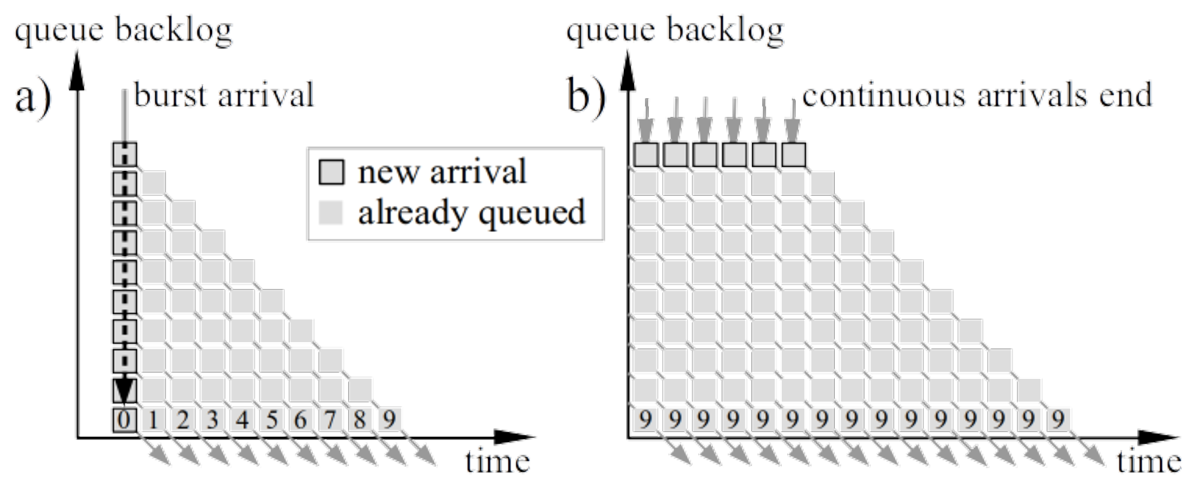
\includegraphics[width=0.8\linewidth]{sojourn-prob}
	\caption{Schematic Illustrating Two Problems with the Sojourn Time Metric. a) It does not measure the full size of a burst until the end (left); b) It does not measure a draining queue (right). Draining is visualized at one equisized packet per timeslot. Sojourn time is represented just before each packet is dequeued as the number of timeslots along its diagonal path.}\label{fig:sojourn-prob}
\end{figure*}

Control path delay consists of the following elements:
\begin{itemize}[nosep]
	\item propagation delay (in common with the data);
	\item queuing delay (in common with the data);
	\item measurement delay: measuring the queue, as well as arrival and/or departure rates;
	\item smoothing delay: filtering out fluctuations in measurements;
	\item signal encoding delay: a number representing the signal is produced within an AQM algorithm, which is then compressed into a unary `encoding' in each packet, and `decoded' by the congestion control algorithm's response to the unary-encoded signals. A unary encoding is used so that the AQM does not have to recognize flows or hold per-flow state. But it constrains the bandwidth of the signalling channel, which introduces encoding delay;
	\item randomization delay: randomness is introduced to break up oscillations, but it requires longer to detect the underlying signal.
\end{itemize}

This memo pays most attention to two of these: measurement and queuing delay. The other four are briefly surveyed in \S\,\ref{sec:related}.

% ================================================================
\section{The Problem}\label{sigqdyntr_problem}
% ----------------------------------------------------------------
\subsection{The Problem in Brief}\label{sigqdyntr_problem_brief}
The signal from an AQM can be subject to unnecessary \textbf{queuing delay} if it is applied to a packet during the enqueue process, so that it has to work its way through the queue before being transmitted to the line. In classical AQMs, queuing delay is configured to be of the same order of magnitude as typical propagation delays. Therefore subjecting the congestion signal to the delay of the queue will add unnecessary sloppiness to the control loop.

Even if a signal is applied to a packet as it is dequeued, it is often based on a \textbf{measurement} that has taken some time to collect. For instance, the sojourn time technique, which is becoming common for measuring the queue in modern AQMs, gives a queue delay metric that is always out of date by the amount of time the packet spent in the queue. So even if the signal is applied at dequeue, it is delayed by the time spent measuring it in the queue.

The sojourn time measured when a packet reaches the head of the queue takes no account of any change in the queue while that packet is working towards the head. Despite the queuing system holding all the information about those recent changes. So if a burst arrives, the sojourn time of packets in front of the burst will show no evidence of the queue building behind them. For instance, in \autoref{fig:sojourn-prob}a), the sojourn of the first packet of the burst takes '0' timeslots. And the sojourn time metric only fully measures the burst when the last packet of the burst reaches the head of the queue, where '9' is shown. Even though, in this case, all the packets of the burst had arrived before the packet tagged '1' was dequeued. In \S\,\ref{sec:fairer_marking} we will consider a mix of smooth and bursty traffic, then we will see how this delay attributing blame for a burst tends to shift the blame from bursty to smooth traffic.

Whenever the drain rate abruptly reduces, use of sojourn time is similarly problematic. As soon as the reduction occurs, the time that packets will take to work through the queue increases. But, the sojourn time of those packets that have already worked their way towards the head of the queue does not reflect the delay that will be experienced by the packets behind them.

Conversely, consider the queue in \autoref{fig:sojourn-prob}b) that has been stable then the data flow ends abruptly, so that no further packets arrive. Then, even when the last packet to arrive is about to be dequeued from the head of the queue, its sojourn time still measures the stable queue delay when it arrived, because that's how long it took to drain the queue. If sojourn alone were used for marking and dropping, there would be no externally visible evidence of the now empty queue behind the last packet until traffic started again.

Implementations of AQMs that use sojourn time sometimes include code to deal with certain exceptional cases (such as an empty queue). But this memo proposes simple techniques to cut out the root cause of that measurement delay in all cases; by using all the information available in the queue at the point that a packet is dequeued. At dequeue there is very little time for additional processing, so considerable attention has had to be paid to minimizing execution time as well.
